% Options for packages loaded elsewhere
\PassOptionsToPackage{unicode}{hyperref}
\PassOptionsToPackage{hyphens}{url}
%
\documentclass[
]{article}
\usepackage{lmodern}
\usepackage{amssymb,amsmath}
\usepackage{ifxetex,ifluatex}
\ifnum 0\ifxetex 1\fi\ifluatex 1\fi=0 % if pdftex
  \usepackage[T1]{fontenc}
  \usepackage[utf8]{inputenc}
  \usepackage{textcomp} % provide euro and other symbols
\else % if luatex or xetex
  \usepackage{unicode-math}
  \defaultfontfeatures{Scale=MatchLowercase}
  \defaultfontfeatures[\rmfamily]{Ligatures=TeX,Scale=1}
\fi
% Use upquote if available, for straight quotes in verbatim environments
\IfFileExists{upquote.sty}{\usepackage{upquote}}{}
\IfFileExists{microtype.sty}{% use microtype if available
  \usepackage[]{microtype}
  \UseMicrotypeSet[protrusion]{basicmath} % disable protrusion for tt fonts
}{}
\makeatletter
\@ifundefined{KOMAClassName}{% if non-KOMA class
  \IfFileExists{parskip.sty}{%
    \usepackage{parskip}
  }{% else
    \setlength{\parindent}{0pt}
    \setlength{\parskip}{6pt plus 2pt minus 1pt}}
}{% if KOMA class
  \KOMAoptions{parskip=half}}
\makeatother
\usepackage{xcolor}
\IfFileExists{xurl.sty}{\usepackage{xurl}}{} % add URL line breaks if available
\IfFileExists{bookmark.sty}{\usepackage{bookmark}}{\usepackage{hyperref}}
\hypersetup{
  pdftitle={Numerical trajectory patterns of floating macroalgae},
  pdfauthor={R Coppin; C Rautenbach; AJ Smit},
  hidelinks,
  pdfcreator={LaTeX via pandoc}}
\urlstyle{same} % disable monospaced font for URLs
\usepackage[margin=1in]{geometry}
\usepackage{graphicx,grffile}
\makeatletter
\def\maxwidth{\ifdim\Gin@nat@width>\linewidth\linewidth\else\Gin@nat@width\fi}
\def\maxheight{\ifdim\Gin@nat@height>\textheight\textheight\else\Gin@nat@height\fi}
\makeatother
% Scale images if necessary, so that they will not overflow the page
% margins by default, and it is still possible to overwrite the defaults
% using explicit options in \includegraphics[width, height, ...]{}
\setkeys{Gin}{width=\maxwidth,height=\maxheight,keepaspectratio}
% Set default figure placement to htbp
\makeatletter
\def\fps@figure{htbp}
\makeatother
\setlength{\emergencystretch}{3em} % prevent overfull lines
\providecommand{\tightlist}{%
  \setlength{\itemsep}{0pt}\setlength{\parskip}{0pt}}
\setcounter{secnumdepth}{-\maxdimen} % remove section numbering
\usepackage{fontspec}
\usepackage{multirow}
\usepackage{multicol}
\usepackage{colortbl}
\usepackage{hhline}
\usepackage{longtable}
\usepackage{array}
\usepackage{hyperref}

\title{Numerical trajectory patterns of floating macroalgae}
\author{R Coppin\footnote{University of the Western Cape} \and C Rautenbach\footnote{South African Weather Service} \and AJ Smit\footnote{University of the Western Cape}}
\date{}

\begin{document}
\maketitle

\hypertarget{introduction}{%
\section{Introduction}\label{introduction}}

There is a range of objects, both natural and anthropogenic, floating in
the ocean of which macroalgae are regarded as one of the most important
passive dispersal mechanisms of marine taxa. Floating kelp acts as a
passive dispersal mechanism for a range of marine taxa and is sometimes
referred to as the `tumble-weed' of the ocean (Edgar, 1987; Norton,
1992; Bushing, 1994; Helmuth et al., 1994; Holmquist, 1994; Smith, 2002;
McCormick et al., 2008). Some macroalgae species are negatively buoyant
and sink to the seafloor when detached from the substrate, while other
species of macroalgae have air-filled pneumatocysts or stipes which
allow the plants to reach the surface where light is more abundant. In
turn, the positively buoyant pneumatocysts cause plants to float to the
surface when dislodged from the substratum. The structure and number of
pneumatocysts varies between species. For example species from the
genera \emph{Macrocystis}, \emph{Sargassum}, \emph{Ascophyllum}, and
\emph{Fucus} have thalli with many small pneumatocysts, while other kelp
species such as \emph{Nereocystis luetkeana}, \emph{Pelagophycus porra},
\emph{Ecklonia radiata}, \emph{Ecklonia maxima} have a single, large
pneumatocysts (Dayton, 1985; Smith, 2002; Thiel and Gutow, 2005; Graiff
et al., 2016; Batista et al., 2018). In some cases the stipe itself is
air-filled, such as with \emph{E. maxima} and \emph{E. radiata}.
Although there have been reports of floating Chlorophyta species and
some Rhodophyta species, Phaeophyceae species are the most commonly
reported forms of floating algae. This is most likely because the green
and red species reported floating are not actually positively buoyant,
but instead are kept at the surface by gas trapped inbetween or in the
thalli (Dromgoole, 1982; Bäck et al., 2000). The giant kelp
\emph{Macrocystis pyrifera} (Helmuth et al., 1994; Kingsford, 1995;
Hobday, 2000; Macaya et al., 2005; Graiff et al., 2016; Batista et al.,
2018) and the bull kelp \emph{Durvillaea antarctica} (Smith, 2002;
Collins et al., 2010; Wichmann et al., 2012; Tala et al., 2013 , 2017;
Saunders, 2014; Batista et al., 2018) have been the focus of much of the
research regarding spatial and temporal dispersal patterns, the
ecological role of rafting, marine connectivity and raft-time.

Past research points to macroalgae trajectory being largely determined
by prevailing wind conditions and surface currents (Hobday, 2000; Thiel
and Gutow, 2005, @thiel2005; Fraser et al., 2011; Rothäusler et al.,
2011, 2011). Although ocean currents are regarded as the primary
influence, the relative importance of wind versus surface current is
still not known; although the role of wind has been recognised as
important in several studies. For example, a study by Harrold and Lisin
(1989) investigated the seasonal trajectories of radio-transmitter
tagged \emph{M. pyrifera} in nearshore Monterrey Bay. The results showed
that kelp rafts with little surface area exposed to the wind were
largely driven by a combination of wind and wind waves, however the
relative importance of wind and wind waves was not clear. In addition,
the tagged kelp trajectories were more consistent with the formation of
eddies during winter. Previous studies have identified wind as an
important mechanism of dispersal in wind dominated ocean systems. For
example the subAntartic latitudes the West Wind Drift causes continuous
unidirectional surface flow and is regarded as an important potential
mechanism for dispersal of floating kelp. Other studies have used
genetic approaches to determine macroalgae raft trajectory
characteristics by inferring source location from genetically similar
populations (Nikula et al., 2013). For example, a study by Fraser et al.
(2011) on the rafting capabilities of \emph{Durvillaea antarctica} used
a combination of population genetics and relative age estimate of
`goosebarnacles' attached to the raft. The presence of goosebarnacles
suggests a long raft time as these species have a slow growth rate;
while the genetic analyses showed these species are able to raft up to
\(\sim\) 390km from their local origin. The authors suggested that wind
and water-movement were the primary influences of trajectory, however,
this was only inferred from the genetic results and local climatology
data (Fraser et al., 2011).

Other aspects such as buoyancy and drag also play a role in determining
the trajectory and rate of transport for surface floating material.
However, the past research on macroalgal trajectory has not investigated
these factors which have been shown to be important aspects of
trajectory for other materials such as icebergs, marine craft and
microplastics. The ``sail'' area of an object floating at sea is the
surface area exposed to the wind which results in air form drag, while
the area of the object below the surface of the water is exposed to
surface currents which result in hydrodynamic form drag. Drag
coefficients related to wind and surface current have been shown to be
important properties to consider when estimating trajectory and
forecasting drift for search and sea rescue operations. Drag is
ultimately determined by the size and shape of the object which are
properties that vary considerably with macroalgae species. In addition,
past research conducted within the maritime industry has shown that the
size and shape of a vessel determine the relative importance of waves or
wind as drivers of trajectory, as well as orientation of the object. If
the length of the object is longer than the significant wave height then
waves will be the primary driver of trajectory while the opposite is
true for smaller objects where the effect of waves is regarded as
negligible (Breivik et al., 2011; Griffin et al., 2017).

To accurately determine the trajectory of marine macroalgae these
aspects need to be taken into account. Past research by Allen and
Plourde (1999) and Breivik et al. (2011) have provided estimates of drag
for various objects based on experimental work, which consisted of both
direct and indirect methods of the Leeway model. However, this work does
not consider biological material such as macroalgae. Although drag
estimates do exist, these have been applied for macroalgae not detached
from the substratum and are regarded as fixed-point estimates. Although
various approaches have been used in the past to investigate floating
macroalagae trajectory, very few studies have employed the use of
Langrangian trajectory modeling. Furthermore, non of the existing
studies using this modeling approach have considered macroalgal
morphology cross-sectional area (i.e.~shape) as an aspect of drag and
ultimately trajectory. Studies by Brooks et al. (2019), Putman et al.
(2018), Putman et al. (2020) used lagrangian approaches to investigate
the effects of inertia, raft-size, and windage on macroalgae trajectory.
Brooks et al. (2019) used a custom growth model to estimate changes in
biomass and ultimately radial size, while a customised Hybrid Coordinate
Ocean Model (HYCOM) for the trajectory simulations was used. The results
showed that trajectory of pelagic \emph{Sargussum} was significantly
influenced by inertia and the radial size of the rafts. Other work by
Putman et al. (2020) investigated the effect of including windage in
macroalgae trajectory simulations. The authors showed that including
ad-hoc windage factors greatly improved accuracy regarding entrainment
or expulsion from eddies when compared to tracked sargassum mats in the
ocean. Langrangian trajectory modeling is a useful tool, however, the
various models available often assume the object to be a spherical
particle, which is obviously not the case for both biological and
anthropogenic forms of marine debris in nature. The radial size included
by Brooks et al. (2019) is an improvement, however this approach does
not take into account the complex morphology on an individual level into
account.

In this study, a numerical approach is used to shed light on the role of
hydrodynamic and direct wind drag on macroalgal drift trajectory using
lagrangian based trajectory simulations. This will be achieved by
comparing the trajectory outputs of virtual `passive' particles (no drag
characteristics added) with kelp particles (drag characteristics added)
of varying degrees of hydrodynamic and wind drag exposure. The different
degrees of wave and wind exposure are meant to reflect the different
buoyancy characteristics, as well as identify the role of magnitude of
the drag components on overall trajectory.

\hypertarget{methods}{%
\section{Methods}\label{methods}}

\hypertarget{study-site}{%
\subsection{Study site}\label{study-site}}

The region of interest for this study was the Cape Peninsula in the
Western Cape (Figure 1A). A release site was chosen for this study,
Kommetjie, which is located on the Atlantic side of the Cape Peninsula
(Figure 2B). The hydrodynamics in the study region are driven by a
complex interaction of wind and waves. which are also influenced by
larger oceanic processes In South Africa, the larger processes can
largely be attributed to the Agulhas Current (AC) and the Benguela
Current (BC). The AC is a component of the South-west Indian Ocean
sub-gyre, flowing predominantly south-westward following the continental
shelf edge and eventually retroflecting eastward back into the South
Indian Ocean. The region where the retroflection occurs is known as the
Agulhas retroflection and consists of some of the highest levels of
mesoscale variability (Garzoli et al., 1996). The variability results in
shedding of rings and filaments known as the Agulhas Rings and have an
average diameter of \textasciitilde324km (Lutjeharms and Van
Ballegooyen, 1988; Lutjeharms, 2006, @ 2007). The Agulhas Rings are the
main contributors to the Agulhas leakage which is the transport of warm
water from the Indian Ocean to the South Atlantic Ocean (Garzoli et al.,
1996; Lutjeharms, 2006; Beal et al., 2015). The Agulhas leakage is also
a source of meso-scale variability within the Benguela region as
anticyclonic rings are shed and drift northwestward along the southern
Benguela slope region (Rubio et al., 2009). The Benguela region is
characterised by strong coastal upwelling cells which a primarily driven
by equatorward winds (Shannon and Nelson, 1996; Hardman-Mountford et
al., 2003), and is known as the Benguela upwelling region. The Benguela
upwelling region starts at 27\(^\circ\)S and extends southward to
35\(^\circ\)S (Shannon and Nelson, 1996). The region is also
characterised by high amounts of mesoscale variability in the form of
eddies and filaments(Blanke et al., 2002, 2005; Rubio et al., 2009). The
Benguela inshore region is dominated by a northwestward flow as a result
of topographical steering, wind stress and interactions with passing
Agulhas rings and eddies (Veitch et al., 2010).

\begin{figure}
\centering
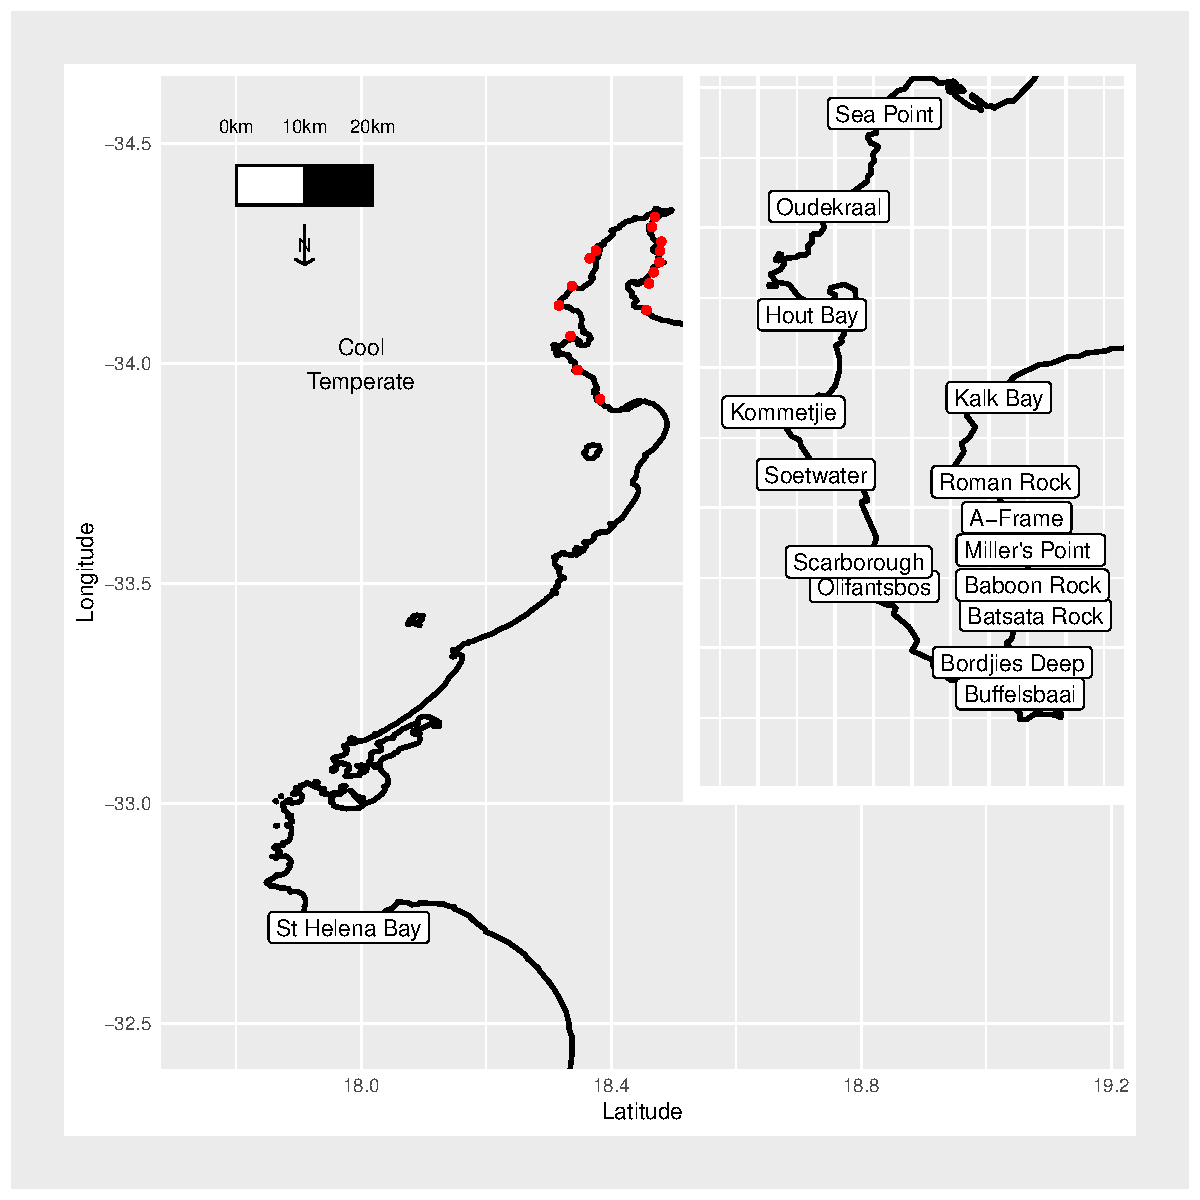
\includegraphics{thesis_chapter_3_files/figure-latex/map-1.pdf}
\caption{Figure 1:Map of the study domain. This is a temporary map until
issues with the map script are resolved.}
\end{figure}

\hypertarget{particle-tracking-model}{%
\subsection{Particle tracking model}\label{particle-tracking-model}}

The model is based on parameterisations that have been used for previous
studies investigating iceberg, capsized marine vessels and
microplastics. It should be noted that most of the previous studies
regarding macroalgae trajectory have investigated rafts and not solitary
floating individuals. A kelp raft will vary in size and can range from a
few meters across to large dense mats the size of a sports field.
Furthermore, some authors suggest that most macroalgae become entangled
through ocean currents and not through the hydrodynamic forces that
dislodge them. In addition, large kelp rafts are not a characteristics
around the coast of the Cape Peninsula but rather solitary kelp are
(Pers. Obs). Therefore, the trajectory of only solitary \emph{E. maxima}
individuals will be considered. Numerical calculations of particle
trajectory with a Lagrangian method (Delandmeter and Van Sebille, 2019),
and be described by the equation

\[X(t+\Delta t) = X(t) + \int_{t}^{t+\Delta t} v(x, \tau)d \tau + \Delta X_b(t)\]
where \(X\) is the three-dimensional position of a particle, \(v(x,t)\)
is the three-dimensional velocity field at the location in the ocean
model, \(X_b(t)\) is a change in position due to `behavior' of the
particle. This can range from swimming in fish to sinking or beaching.
IN order to investigate the effects of drag components of trajectory of
floating macroalgae, this study incorporated drag as the custom
behavior.

This study simulated two scenarios; one where the plant is fully
submerged and only exposed to hydrodynamic drag; and the other where
parts of the plants are partially exposed resulting in a combination of
hydrodynamic and air form drag. Drag based on shape based coefficients
were used in the calculations for determining the overall kelp velocity
vectors. A momentum energy equation was used to calculate the drag
forces for the relevant simulation. This approach has been employed in
modeling iceberg drift trajectory (Lichey and Hellmer, 2001; Eik, 2009;
Andersson et al., 2017) and was adapted to suit this particular study.
The energy momentum equation used to calculate the drag force exerted on
the virtual kelp particle was, \[m({d_u/d_t})=F_d + F_a + F_f\] where
\(m\) is kelp mass, \(d_u\) the virtual kelp particle velocity, \(F_d\)
the hydrodynamic drag, \(F_a\) is the wind drag, and \(F_f\) the
surface-current flow. The assumption made was that the mass of the kelp
did not change for each virtual kelp particle over the course of the
simulations. Hydrodynamic drag, wind drag and surface current-flow are
two-dimensional vector quantities and were calculated for each time step
for each simulation.

\hypertarget{hydrodynamic-and-wind-model}{%
\subsection{Hydrodynamic and wind
model}\label{hydrodynamic-and-wind-model}}

Both passive and kelp particles were simulated around the South African
coastline within hind-cast outputs from the Copernicus Marine
Environment Monitoring Service. The Copernicus outputs used in this
study contains 3D daily current information from the top layer to the
bottom (Global Analysis Forecast PHY\_001\_024). The model has a spatial
resolution of 0.08\(^\circ\) and is interpolated on a Arakawa C native
grid.

In order to incorporate the effects of direct wind drag within the
simulations, the Copernicus Marine Environment Monitoring Service global
wind product was used (WIND\_L4\_NRT\_OBSERVATIONS\_012\_004). The
outputs from the model is composed of 6-hourly averaged fields of
surface 10m wind velocity vectors with a spatial resolution of
0.25\(^\circ\). Both averaged ocean current and wind data are stored as
meridonal and zonal velocity vectors.

\hypertarget{simulations}{%
\subsection{Simulations}\label{simulations}}

Virtual particles were released with no drag or wind effects from the
study site in order to act as a basis for comparison to simulations with
varying degrees of hydrodynamic and wind drag, and are referred to
hereafter as `passive particles'. All simulations have the same release
location and were run for 30 days with hourly outputs using a fourth
order Runge-Kutte advection scheme. Brownian motion was also
incorporated in order to account for any stochasticity not resolved by
the model. These are standard practices for Lagrangian trajectory
studies.

\providecommand{\docline}[3]{\noalign{\global\setlength{\arrayrulewidth}{#1}}\arrayrulecolor[HTML]{#2}\cline{#3}}

\setlength{\tabcolsep}{8pt}

\renewcommand*{\arraystretch}{1.5}

\begin{table}

\centering

\begin{longtable}{ccccc}

\caption{Table 1:Details for each simulation executed for the study.}\\

\hhline{~~~~~}

\multicolumn{1}{!{\color[HTML]{000000}\vrule width 0pt}>{}c}{\fontsize{11}{13}\selectfont{\textcolor[HTML]{000000}{\textbf{Scenario}}}} & \multicolumn{1}{!{\color[HTML]{000000}\vrule width 0pt}>{}c}{\fontsize{11}{13}\selectfont{\textcolor[HTML]{000000}{\textbf{ID}}}} & \multicolumn{1}{!{\color[HTML]{000000}\vrule width 0pt}>{}c}{\fontsize{11}{13}\selectfont{\textcolor[HTML]{000000}{\textbf{Type}}}} & \multicolumn{1}{!{\color[HTML]{000000}\vrule width 0pt}>{}c}{\fontsize{11}{13}\selectfont{\textcolor[HTML]{000000}{\textbf{Cross-sectional area}}}} & \multicolumn{1}{!{\color[HTML]{000000}\vrule width 0pt}>{}c!{\color[HTML]{000000}\vrule width 0pt}}{\fontsize{11}{13}\selectfont{\textcolor[HTML]{000000}{\textbf{Drag Exposure level}}}} \\



\endfirsthead

\hhline{~~~~~}

\multicolumn{1}{!{\color[HTML]{000000}\vrule width 0pt}>{}c}{\fontsize{11}{13}\selectfont{\textcolor[HTML]{000000}{\textbf{Scenario}}}} & \multicolumn{1}{!{\color[HTML]{000000}\vrule width 0pt}>{}c}{\fontsize{11}{13}\selectfont{\textcolor[HTML]{000000}{\textbf{ID}}}} & \multicolumn{1}{!{\color[HTML]{000000}\vrule width 0pt}>{}c}{\fontsize{11}{13}\selectfont{\textcolor[HTML]{000000}{\textbf{Type}}}} & \multicolumn{1}{!{\color[HTML]{000000}\vrule width 0pt}>{}c}{\fontsize{11}{13}\selectfont{\textcolor[HTML]{000000}{\textbf{Cross-sectional area}}}} & \multicolumn{1}{!{\color[HTML]{000000}\vrule width 0pt}>{}c!{\color[HTML]{000000}\vrule width 0pt}}{\fontsize{11}{13}\selectfont{\textcolor[HTML]{000000}{\textbf{Drag Exposure level}}}} \\

\endhead



\multicolumn{1}{!{\color[HTML]{000000}\vrule width 0pt}>{\cellcolor[HTML]{EFEFEF}}c}{\fontsize{11}{13}\selectfont{\textcolor[HTML]{000000}{1}}} & \multicolumn{1}{!{\color[HTML]{000000}\vrule width 0pt}>{\cellcolor[HTML]{EFEFEF}}c}{\fontsize{11}{13}\selectfont{\textcolor[HTML]{000000}{RK4\_Pfloat}}} & \multicolumn{1}{!{\color[HTML]{000000}\vrule width 0pt}>{\cellcolor[HTML]{EFEFEF}}c}{\fontsize{11}{13}\selectfont{\textcolor[HTML]{000000}{Passive}}} & \multicolumn{1}{!{\color[HTML]{000000}\vrule width 0pt}>{\cellcolor[HTML]{EFEFEF}}c}{\fontsize{11}{13}\selectfont{\textcolor[HTML]{000000}{N/A}}} & \multicolumn{1}{!{\color[HTML]{000000}\vrule width 0pt}>{\cellcolor[HTML]{EFEFEF}}c!{\color[HTML]{000000}\vrule width 0pt}}{\fontsize{11}{13}\selectfont{\textcolor[HTML]{000000}{N/A}}} \\





\multicolumn{1}{!{\color[HTML]{000000}\vrule width 0pt}>{}c}{\fontsize{11}{13}\selectfont{\textcolor[HTML]{000000}{2}}} & \multicolumn{1}{!{\color[HTML]{000000}\vrule width 0pt}>{}c}{\fontsize{11}{13}\selectfont{\textcolor[HTML]{000000}{Min\_Kfloat\_H100W00}}} & \multicolumn{1}{!{\color[HTML]{000000}\vrule width 0pt}>{}c}{\fontsize{11}{13}\selectfont{\textcolor[HTML]{000000}{Kelp}}} & \multicolumn{1}{!{\color[HTML]{000000}\vrule width 0pt}>{}c}{\fontsize{11}{13}\selectfont{\textcolor[HTML]{000000}{Minimum}}} & \multicolumn{1}{!{\color[HTML]{000000}\vrule width 0pt}>{}c!{\color[HTML]{000000}\vrule width 0pt}}{\fontsize{11}{13}\selectfont{\textcolor[HTML]{000000}{Hydrodynamic drag only}}} \\





\multicolumn{1}{!{\color[HTML]{000000}\vrule width 0pt}>{\cellcolor[HTML]{EFEFEF}}c}{\fontsize{11}{13}\selectfont{\textcolor[HTML]{000000}{3}}} & \multicolumn{1}{!{\color[HTML]{000000}\vrule width 0pt}>{\cellcolor[HTML]{EFEFEF}}c}{\fontsize{11}{13}\selectfont{\textcolor[HTML]{000000}{Min\_Kfloat\_H095W005}}} & \multicolumn{1}{!{\color[HTML]{000000}\vrule width 0pt}>{\cellcolor[HTML]{EFEFEF}}c}{\fontsize{11}{13}\selectfont{\textcolor[HTML]{000000}{Kelp}}} & \multicolumn{1}{!{\color[HTML]{000000}\vrule width 0pt}>{\cellcolor[HTML]{EFEFEF}}c}{\fontsize{11}{13}\selectfont{\textcolor[HTML]{000000}{Minimum}}} & \multicolumn{1}{!{\color[HTML]{000000}\vrule width 0pt}>{\cellcolor[HTML]{EFEFEF}}c!{\color[HTML]{000000}\vrule width 0pt}}{\fontsize{11}{13}\selectfont{\textcolor[HTML]{000000}{Hydrodynamic drag 95\%, wind drag 5\%}}} \\





\multicolumn{1}{!{\color[HTML]{000000}\vrule width 0pt}>{}c}{\fontsize{11}{13}\selectfont{\textcolor[HTML]{000000}{4}}} & \multicolumn{1}{!{\color[HTML]{000000}\vrule width 0pt}>{}c}{\fontsize{11}{13}\selectfont{\textcolor[HTML]{000000}{Min\_Kfloat\_H090W10}}} & \multicolumn{1}{!{\color[HTML]{000000}\vrule width 0pt}>{}c}{\fontsize{11}{13}\selectfont{\textcolor[HTML]{000000}{Kelp}}} & \multicolumn{1}{!{\color[HTML]{000000}\vrule width 0pt}>{}c}{\fontsize{11}{13}\selectfont{\textcolor[HTML]{000000}{Minimum}}} & \multicolumn{1}{!{\color[HTML]{000000}\vrule width 0pt}>{}c!{\color[HTML]{000000}\vrule width 0pt}}{\fontsize{11}{13}\selectfont{\textcolor[HTML]{000000}{Hydrodynamic drag 90\%, wind drag 10\%}}} \\





\multicolumn{1}{!{\color[HTML]{000000}\vrule width 0pt}>{\cellcolor[HTML]{EFEFEF}}c}{\fontsize{11}{13}\selectfont{\textcolor[HTML]{000000}{5}}} & \multicolumn{1}{!{\color[HTML]{000000}\vrule width 0pt}>{\cellcolor[HTML]{EFEFEF}}c}{\fontsize{11}{13}\selectfont{\textcolor[HTML]{000000}{Min\_Kfloat\_H085W15}}} & \multicolumn{1}{!{\color[HTML]{000000}\vrule width 0pt}>{\cellcolor[HTML]{EFEFEF}}c}{\fontsize{11}{13}\selectfont{\textcolor[HTML]{000000}{Kelp}}} & \multicolumn{1}{!{\color[HTML]{000000}\vrule width 0pt}>{\cellcolor[HTML]{EFEFEF}}c}{\fontsize{11}{13}\selectfont{\textcolor[HTML]{000000}{Minimum}}} & \multicolumn{1}{!{\color[HTML]{000000}\vrule width 0pt}>{\cellcolor[HTML]{EFEFEF}}c!{\color[HTML]{000000}\vrule width 0pt}}{\fontsize{11}{13}\selectfont{\textcolor[HTML]{000000}{Hydrodynamic drag 85\%, wind drag 15\%}}} \\





\multicolumn{1}{!{\color[HTML]{000000}\vrule width 0pt}>{}c}{\fontsize{11}{13}\selectfont{\textcolor[HTML]{000000}{6}}} & \multicolumn{1}{!{\color[HTML]{000000}\vrule width 0pt}>{}c}{\fontsize{11}{13}\selectfont{\textcolor[HTML]{000000}{Mean\_Kfloat\_H100W00}}} & \multicolumn{1}{!{\color[HTML]{000000}\vrule width 0pt}>{}c}{\fontsize{11}{13}\selectfont{\textcolor[HTML]{000000}{Kelp}}} & \multicolumn{1}{!{\color[HTML]{000000}\vrule width 0pt}>{}c}{\fontsize{11}{13}\selectfont{\textcolor[HTML]{000000}{Mean}}} & \multicolumn{1}{!{\color[HTML]{000000}\vrule width 0pt}>{}c!{\color[HTML]{000000}\vrule width 0pt}}{\fontsize{11}{13}\selectfont{\textcolor[HTML]{000000}{Hydrodynamic drag only}}} \\





\multicolumn{1}{!{\color[HTML]{000000}\vrule width 0pt}>{\cellcolor[HTML]{EFEFEF}}c}{\fontsize{11}{13}\selectfont{\textcolor[HTML]{000000}{7}}} & \multicolumn{1}{!{\color[HTML]{000000}\vrule width 0pt}>{\cellcolor[HTML]{EFEFEF}}c}{\fontsize{11}{13}\selectfont{\textcolor[HTML]{000000}{Mean\_Kfloat\_H095W005}}} & \multicolumn{1}{!{\color[HTML]{000000}\vrule width 0pt}>{\cellcolor[HTML]{EFEFEF}}c}{\fontsize{11}{13}\selectfont{\textcolor[HTML]{000000}{Kelp}}} & \multicolumn{1}{!{\color[HTML]{000000}\vrule width 0pt}>{\cellcolor[HTML]{EFEFEF}}c}{\fontsize{11}{13}\selectfont{\textcolor[HTML]{000000}{Mean}}} & \multicolumn{1}{!{\color[HTML]{000000}\vrule width 0pt}>{\cellcolor[HTML]{EFEFEF}}c!{\color[HTML]{000000}\vrule width 0pt}}{\fontsize{11}{13}\selectfont{\textcolor[HTML]{000000}{Hydrodynamic drag 95\%, wind drag 5\%}}} \\





\multicolumn{1}{!{\color[HTML]{000000}\vrule width 0pt}>{}c}{\fontsize{11}{13}\selectfont{\textcolor[HTML]{000000}{8}}} & \multicolumn{1}{!{\color[HTML]{000000}\vrule width 0pt}>{}c}{\fontsize{11}{13}\selectfont{\textcolor[HTML]{000000}{Mean\_Kfloat\_H090W10}}} & \multicolumn{1}{!{\color[HTML]{000000}\vrule width 0pt}>{}c}{\fontsize{11}{13}\selectfont{\textcolor[HTML]{000000}{Kelp}}} & \multicolumn{1}{!{\color[HTML]{000000}\vrule width 0pt}>{}c}{\fontsize{11}{13}\selectfont{\textcolor[HTML]{000000}{Mean}}} & \multicolumn{1}{!{\color[HTML]{000000}\vrule width 0pt}>{}c!{\color[HTML]{000000}\vrule width 0pt}}{\fontsize{11}{13}\selectfont{\textcolor[HTML]{000000}{Hydrodynamic drag 90\%, wind drag 10\%}}} \\





\multicolumn{1}{!{\color[HTML]{000000}\vrule width 0pt}>{\cellcolor[HTML]{EFEFEF}}c}{\fontsize{11}{13}\selectfont{\textcolor[HTML]{000000}{9}}} & \multicolumn{1}{!{\color[HTML]{000000}\vrule width 0pt}>{\cellcolor[HTML]{EFEFEF}}c}{\fontsize{11}{13}\selectfont{\textcolor[HTML]{000000}{Mean\_Kfloat\_H085W15}}} & \multicolumn{1}{!{\color[HTML]{000000}\vrule width 0pt}>{\cellcolor[HTML]{EFEFEF}}c}{\fontsize{11}{13}\selectfont{\textcolor[HTML]{000000}{Kelp}}} & \multicolumn{1}{!{\color[HTML]{000000}\vrule width 0pt}>{\cellcolor[HTML]{EFEFEF}}c}{\fontsize{11}{13}\selectfont{\textcolor[HTML]{000000}{Mean}}} & \multicolumn{1}{!{\color[HTML]{000000}\vrule width 0pt}>{\cellcolor[HTML]{EFEFEF}}c!{\color[HTML]{000000}\vrule width 0pt}}{\fontsize{11}{13}\selectfont{\textcolor[HTML]{000000}{Hydrodynamic drag 85\%, wind drag 15\%}}} \\





\multicolumn{1}{!{\color[HTML]{000000}\vrule width 0pt}>{}c}{\fontsize{11}{13}\selectfont{\textcolor[HTML]{000000}{10}}} & \multicolumn{1}{!{\color[HTML]{000000}\vrule width 0pt}>{}c}{\fontsize{11}{13}\selectfont{\textcolor[HTML]{000000}{Max\_Kfloat\_H100W00}}} & \multicolumn{1}{!{\color[HTML]{000000}\vrule width 0pt}>{}c}{\fontsize{11}{13}\selectfont{\textcolor[HTML]{000000}{Kelp}}} & \multicolumn{1}{!{\color[HTML]{000000}\vrule width 0pt}>{}c}{\fontsize{11}{13}\selectfont{\textcolor[HTML]{000000}{Maximum}}} & \multicolumn{1}{!{\color[HTML]{000000}\vrule width 0pt}>{}c!{\color[HTML]{000000}\vrule width 0pt}}{\fontsize{11}{13}\selectfont{\textcolor[HTML]{000000}{Hydrodynamic drag only}}} \\





\multicolumn{1}{!{\color[HTML]{000000}\vrule width 0pt}>{\cellcolor[HTML]{EFEFEF}}c}{\fontsize{11}{13}\selectfont{\textcolor[HTML]{000000}{11}}} & \multicolumn{1}{!{\color[HTML]{000000}\vrule width 0pt}>{\cellcolor[HTML]{EFEFEF}}c}{\fontsize{11}{13}\selectfont{\textcolor[HTML]{000000}{Max\_Kfloat\_H095W005}}} & \multicolumn{1}{!{\color[HTML]{000000}\vrule width 0pt}>{\cellcolor[HTML]{EFEFEF}}c}{\fontsize{11}{13}\selectfont{\textcolor[HTML]{000000}{Kelp}}} & \multicolumn{1}{!{\color[HTML]{000000}\vrule width 0pt}>{\cellcolor[HTML]{EFEFEF}}c}{\fontsize{11}{13}\selectfont{\textcolor[HTML]{000000}{Maximum}}} & \multicolumn{1}{!{\color[HTML]{000000}\vrule width 0pt}>{\cellcolor[HTML]{EFEFEF}}c!{\color[HTML]{000000}\vrule width 0pt}}{\fontsize{11}{13}\selectfont{\textcolor[HTML]{000000}{Hydrodynamic drag 95\%, wind drag 5\%}}} \\





\multicolumn{1}{!{\color[HTML]{000000}\vrule width 0pt}>{}c}{\fontsize{11}{13}\selectfont{\textcolor[HTML]{000000}{12}}} & \multicolumn{1}{!{\color[HTML]{000000}\vrule width 0pt}>{}c}{\fontsize{11}{13}\selectfont{\textcolor[HTML]{000000}{Max\_Kfloat\_H090W10}}} & \multicolumn{1}{!{\color[HTML]{000000}\vrule width 0pt}>{}c}{\fontsize{11}{13}\selectfont{\textcolor[HTML]{000000}{Kelp}}} & \multicolumn{1}{!{\color[HTML]{000000}\vrule width 0pt}>{}c}{\fontsize{11}{13}\selectfont{\textcolor[HTML]{000000}{Maximum}}} & \multicolumn{1}{!{\color[HTML]{000000}\vrule width 0pt}>{}c!{\color[HTML]{000000}\vrule width 0pt}}{\fontsize{11}{13}\selectfont{\textcolor[HTML]{000000}{Hydrodynamic drag 90\%, wind drag 10\%}}} \\





\multicolumn{1}{!{\color[HTML]{000000}\vrule width 0pt}>{\cellcolor[HTML]{EFEFEF}}c}{\fontsize{11}{13}\selectfont{\textcolor[HTML]{000000}{13}}} & \multicolumn{1}{!{\color[HTML]{000000}\vrule width 0pt}>{\cellcolor[HTML]{EFEFEF}}c}{\fontsize{11}{13}\selectfont{\textcolor[HTML]{000000}{Max\_Kfloat\_H085W15}}} & \multicolumn{1}{!{\color[HTML]{000000}\vrule width 0pt}>{\cellcolor[HTML]{EFEFEF}}c}{\fontsize{11}{13}\selectfont{\textcolor[HTML]{000000}{Kelp}}} & \multicolumn{1}{!{\color[HTML]{000000}\vrule width 0pt}>{\cellcolor[HTML]{EFEFEF}}c}{\fontsize{11}{13}\selectfont{\textcolor[HTML]{000000}{Maximum}}} & \multicolumn{1}{!{\color[HTML]{000000}\vrule width 0pt}>{\cellcolor[HTML]{EFEFEF}}c!{\color[HTML]{000000}\vrule width 0pt}}{\fontsize{11}{13}\selectfont{\textcolor[HTML]{000000}{Hydrodynamic drag 85\%, wind drag 15\%}}} \\





\multicolumn{1}{!{\color[HTML]{000000}\vrule width 0pt}>{}c}{\fontsize{11}{13}\selectfont{\textcolor[HTML]{000000}{14}}} & \multicolumn{1}{!{\color[HTML]{000000}\vrule width 0pt}>{}c}{\fontsize{11}{13}\selectfont{\textcolor[HTML]{000000}{Max\_ShapeFloat\_H085W15}}} & \multicolumn{1}{!{\color[HTML]{000000}\vrule width 0pt}>{}c}{\fontsize{11}{13}\selectfont{\textcolor[HTML]{000000}{Kelp}}} & \multicolumn{1}{!{\color[HTML]{000000}\vrule width 0pt}>{}c}{\fontsize{11}{13}\selectfont{\textcolor[HTML]{000000}{Maximum area, cylinder shape}}} & \multicolumn{1}{!{\color[HTML]{000000}\vrule width 0pt}>{}c!{\color[HTML]{000000}\vrule width 0pt}}{\fontsize{11}{13}\selectfont{\textcolor[HTML]{000000}{Hydrodynamic drag only}}} \\



\end{longtable}

\end{table}

In order to determine the influence of cross-sectional area on drag
components, simulations were performed for the minimum, mean and maximum
cross-sectional areas for Kommetjie kelp forest population (Figure 1).
In order to determine the direct effect of wind on trajectory,
simulations were run for varying magnitudes of wind exposure for each
type of cross-sectional area. The virtual particles released with the
hydrodynamic or wind drag components are referred to as `kelp
particles'.

\hypertarget{model-inputs}{%
\subsection{Model inputs}\label{model-inputs}}

\hypertarget{cross-sectional-area}{%
\subsubsection{Cross-sectional area}\label{cross-sectional-area}}

In order to incorporate hydrodynamic and wind drag, the cross-sectional
area of the kelp was calculated first. Known geometric shapes reflecting
the relevant plant sections were used to estimate the surface area for
various parts of the plant, for details please refer to table 2. The
dimensional data needed was estimated in cases were data was not
available for that particular morphological characteristic. The
bulb/pneumatocyst is a highly variable morphological characteristic and
in some cases can appear absent, the same is true for the holdfast.
Therefore, the cross-sectional area of the bulb/pneumatocyst was not
considered in the calculation of overall cross-sectional area. In terms
of the holdfast, a standard cross-sectional area was used for all
simulations. The cross-sectional area calculated was site specific and
the dimensions needed were garnered from morphology data from a previous
study (Coppin et al., 2020). The minimum, mean and maximum were
calculated for each morphological characteristic (see appendix), which
were used for calculating the overall minimum, mean and maximum
cross-sectional areas needed to run the various simulations. The
trajectory of these ``types'' of cross-sectional areas (minimum, mean
and maximum overall cross-sectional area) were used to determine the
influence of drag, both hydrodynamic and wind, on overall trajectory.

\providecommand{\docline}[3]{\noalign{\global\setlength{\arrayrulewidth}{#1}}\arrayrulecolor[HTML]{#2}\cline{#3}}

\setlength{\tabcolsep}{8pt}

\renewcommand*{\arraystretch}{1.5}

\begin{table}

\centering

\begin{longtable}{ccccccc}

\caption{Table 2:Summary of the atrributes and estimates used to calculate the overall surface area of Kommetjie kelp individuals used in the various simulation.}\\

\hhline{~~~~~~~}

\multicolumn{1}{!{\color[HTML]{000000}\vrule width 0pt}>{}c}{\fontsize{11}{13}\selectfont{\textcolor[HTML]{000000}{\textbf{Plant characteristic}}}} & \multicolumn{1}{!{\color[HTML]{000000}\vrule width 0pt}>{}c}{\fontsize{11}{13}\selectfont{\textcolor[HTML]{000000}{\textbf{Approximate shape}}}} & \multicolumn{1}{!{\color[HTML]{000000}\vrule width 0pt}>{}c}{\fontsize{11}{13}\selectfont{\textcolor[HTML]{000000}{\textbf{Equation Used}}}} & \multicolumn{1}{!{\color[HTML]{000000}\vrule width 0pt}>{}c}{\fontsize{11}{13}\selectfont{\textcolor[HTML]{000000}{\textbf{Plant dimensions}}}} & \multicolumn{1}{!{\color[HTML]{000000}\vrule width 0pt}>{}c}{\fontsize{11}{13}\selectfont{\textcolor[HTML]{000000}{\textbf{Ac Minimum}}}} & \multicolumn{1}{!{\color[HTML]{000000}\vrule width 0pt}>{}c}{\fontsize{11}{13}\selectfont{\textcolor[HTML]{000000}{\textbf{Ac Mean}}}} & \multicolumn{1}{!{\color[HTML]{000000}\vrule width 0pt}>{}c!{\color[HTML]{000000}\vrule width 0pt}}{\fontsize{11}{13}\selectfont{\textcolor[HTML]{000000}{\textbf{Ac Maximum}}}} \\



\endfirsthead

\hhline{~~~~~~~}

\multicolumn{1}{!{\color[HTML]{000000}\vrule width 0pt}>{}c}{\fontsize{11}{13}\selectfont{\textcolor[HTML]{000000}{\textbf{Plant characteristic}}}} & \multicolumn{1}{!{\color[HTML]{000000}\vrule width 0pt}>{}c}{\fontsize{11}{13}\selectfont{\textcolor[HTML]{000000}{\textbf{Approximate shape}}}} & \multicolumn{1}{!{\color[HTML]{000000}\vrule width 0pt}>{}c}{\fontsize{11}{13}\selectfont{\textcolor[HTML]{000000}{\textbf{Equation Used}}}} & \multicolumn{1}{!{\color[HTML]{000000}\vrule width 0pt}>{}c}{\fontsize{11}{13}\selectfont{\textcolor[HTML]{000000}{\textbf{Plant dimensions}}}} & \multicolumn{1}{!{\color[HTML]{000000}\vrule width 0pt}>{}c}{\fontsize{11}{13}\selectfont{\textcolor[HTML]{000000}{\textbf{Ac Minimum}}}} & \multicolumn{1}{!{\color[HTML]{000000}\vrule width 0pt}>{}c}{\fontsize{11}{13}\selectfont{\textcolor[HTML]{000000}{\textbf{Ac Mean}}}} & \multicolumn{1}{!{\color[HTML]{000000}\vrule width 0pt}>{}c!{\color[HTML]{000000}\vrule width 0pt}}{\fontsize{11}{13}\selectfont{\textcolor[HTML]{000000}{\textbf{Ac Maximum}}}} \\

\endhead



\multicolumn{1}{!{\color[HTML]{000000}\vrule width 0pt}>{\cellcolor[HTML]{EFEFEF}}c}{\fontsize{11}{13}\selectfont{\textcolor[HTML]{000000}{Secondary blade}}} & \multicolumn{1}{!{\color[HTML]{000000}\vrule width 0pt}>{\cellcolor[HTML]{EFEFEF}}c}{\fontsize{11}{13}\selectfont{\textcolor[HTML]{000000}{Rectangle}}} & \multicolumn{1}{!{\color[HTML]{000000}\vrule width 0pt}>{\cellcolor[HTML]{EFEFEF}}c}{\fontsize{11}{13}\selectfont{\textcolor[HTML]{000000}{Ac = 2lw + 2lh + 2wh}}} & \multicolumn{1}{!{\color[HTML]{000000}\vrule width 0pt}>{\cellcolor[HTML]{EFEFEF}}c}{\fontsize{11}{13}\selectfont{\textcolor[HTML]{000000}{frond length, frond width*,frond thickness*}}} & \multicolumn{1}{!{\color[HTML]{000000}\vrule width 0pt}>{\cellcolor[HTML]{EFEFEF}}c}{\fontsize{11}{13}\selectfont{\textcolor[HTML]{000000}{1,136}}} & \multicolumn{1}{!{\color[HTML]{000000}\vrule width 0pt}>{\cellcolor[HTML]{EFEFEF}}c}{\fontsize{11}{13}\selectfont{\textcolor[HTML]{000000}{1,993}}} & \multicolumn{1}{!{\color[HTML]{000000}\vrule width 0pt}>{\cellcolor[HTML]{EFEFEF}}c!{\color[HTML]{000000}\vrule width 0pt}}{\fontsize{11}{13}\selectfont{\textcolor[HTML]{000000}{2,550}}} \\





\multicolumn{1}{!{\color[HTML]{000000}\vrule width 0pt}>{}c}{\fontsize{11}{13}\selectfont{\textcolor[HTML]{000000}{Primary blade}}} & \multicolumn{1}{!{\color[HTML]{000000}\vrule width 0pt}>{}c}{\fontsize{11}{13}\selectfont{\textcolor[HTML]{000000}{Rhombus}}} & \multicolumn{1}{!{\color[HTML]{000000}\vrule width 0pt}>{}c}{\fontsize{11}{13}\selectfont{\textcolor[HTML]{000000}{Ac = (lxb)/2}}} & \multicolumn{1}{!{\color[HTML]{000000}\vrule width 0pt}>{}c}{\fontsize{11}{13}\selectfont{\textcolor[HTML]{000000}{primary length, primary width}}} & \multicolumn{1}{!{\color[HTML]{000000}\vrule width 0pt}>{}c}{\fontsize{11}{13}\selectfont{\textcolor[HTML]{000000}{96}}} & \multicolumn{1}{!{\color[HTML]{000000}\vrule width 0pt}>{}c}{\fontsize{11}{13}\selectfont{\textcolor[HTML]{000000}{262}}} & \multicolumn{1}{!{\color[HTML]{000000}\vrule width 0pt}>{}c!{\color[HTML]{000000}\vrule width 0pt}}{\fontsize{11}{13}\selectfont{\textcolor[HTML]{000000}{536}}} \\





\multicolumn{1}{!{\color[HTML]{000000}\vrule width 0pt}>{\cellcolor[HTML]{EFEFEF}}c}{\fontsize{11}{13}\selectfont{\textcolor[HTML]{000000}{Bulb/pneomatocyst}}} & \multicolumn{1}{!{\color[HTML]{000000}\vrule width 0pt}>{\cellcolor[HTML]{EFEFEF}}c}{\fontsize{11}{13}\selectfont{\textcolor[HTML]{000000}{Capsule}}} & \multicolumn{1}{!{\color[HTML]{000000}\vrule width 0pt}>{\cellcolor[HTML]{EFEFEF}}c}{\fontsize{11}{13}\selectfont{\textcolor[HTML]{000000}{Ac = 4?r2 + 2?rh}}} & \multicolumn{1}{!{\color[HTML]{000000}\vrule width 0pt}>{\cellcolor[HTML]{EFEFEF}}c}{\fontsize{11}{13}\selectfont{\textcolor[HTML]{000000}{bulb length*, bulb base radius*}}} & \multicolumn{1}{!{\color[HTML]{000000}\vrule width 0pt}>{\cellcolor[HTML]{EFEFEF}}c}{\fontsize{11}{13}\selectfont{\textcolor[HTML]{000000}{628}}} & \multicolumn{1}{!{\color[HTML]{000000}\vrule width 0pt}>{\cellcolor[HTML]{EFEFEF}}c}{\fontsize{11}{13}\selectfont{\textcolor[HTML]{000000}{628}}} & \multicolumn{1}{!{\color[HTML]{000000}\vrule width 0pt}>{\cellcolor[HTML]{EFEFEF}}c!{\color[HTML]{000000}\vrule width 0pt}}{\fontsize{11}{13}\selectfont{\textcolor[HTML]{000000}{628}}} \\





\multicolumn{1}{!{\color[HTML]{000000}\vrule width 0pt}>{}c}{\fontsize{11}{13}\selectfont{\textcolor[HTML]{000000}{Stipe}}} & \multicolumn{1}{!{\color[HTML]{000000}\vrule width 0pt}>{}c}{\fontsize{11}{13}\selectfont{\textcolor[HTML]{000000}{Cylinder}}} & \multicolumn{1}{!{\color[HTML]{000000}\vrule width 0pt}>{}c}{\fontsize{11}{13}\selectfont{\textcolor[HTML]{000000}{Ac = 2?r(r + h)}}} & \multicolumn{1}{!{\color[HTML]{000000}\vrule width 0pt}>{}c}{\fontsize{11}{13}\selectfont{\textcolor[HTML]{000000}{stipe radius from stipe circumference, stipe length}}} & \multicolumn{1}{!{\color[HTML]{000000}\vrule width 0pt}>{}c}{\fontsize{11}{13}\selectfont{\textcolor[HTML]{000000}{9,797}}} & \multicolumn{1}{!{\color[HTML]{000000}\vrule width 0pt}>{}c}{\fontsize{11}{13}\selectfont{\textcolor[HTML]{000000}{19,338}}} & \multicolumn{1}{!{\color[HTML]{000000}\vrule width 0pt}>{}c!{\color[HTML]{000000}\vrule width 0pt}}{\fontsize{11}{13}\selectfont{\textcolor[HTML]{000000}{34,273}}} \\





\multicolumn{1}{!{\color[HTML]{000000}\vrule width 0pt}>{\cellcolor[HTML]{EFEFEF}}c}{\fontsize{11}{13}\selectfont{\textcolor[HTML]{000000}{Holdfast area}}} & \multicolumn{1}{!{\color[HTML]{000000}\vrule width 0pt}>{\cellcolor[HTML]{EFEFEF}}c}{\fontsize{11}{13}\selectfont{\textcolor[HTML]{000000}{Conical frustrum}}} & \multicolumn{1}{!{\color[HTML]{000000}\vrule width 0pt}>{\cellcolor[HTML]{EFEFEF}}c}{\fontsize{11}{13}\selectfont{\textcolor[HTML]{000000}{Ac = ?(R2 + r2) + ?(R+r)?(R-r)2 + h2}}} & \multicolumn{1}{!{\color[HTML]{000000}\vrule width 0pt}>{\cellcolor[HTML]{EFEFEF}}c}{\fontsize{11}{13}\selectfont{\textcolor[HTML]{000000}{top radius*, bottom radius*, height*}}} & \multicolumn{1}{!{\color[HTML]{000000}\vrule width 0pt}>{\cellcolor[HTML]{EFEFEF}}c}{\fontsize{11}{13}\selectfont{\textcolor[HTML]{000000}{640}}} & \multicolumn{1}{!{\color[HTML]{000000}\vrule width 0pt}>{\cellcolor[HTML]{EFEFEF}}c}{\fontsize{11}{13}\selectfont{\textcolor[HTML]{000000}{640}}} & \multicolumn{1}{!{\color[HTML]{000000}\vrule width 0pt}>{\cellcolor[HTML]{EFEFEF}}c!{\color[HTML]{000000}\vrule width 0pt}}{\fontsize{11}{13}\selectfont{\textcolor[HTML]{000000}{640}}} \\





\multicolumn{1}{!{\color[HTML]{000000}\vrule width 0pt}>{}c}{\fontsize{11}{13}\selectfont{\textcolor[HTML]{000000}{}}} & \multicolumn{1}{!{\color[HTML]{000000}\vrule width 0pt}>{}c}{\fontsize{11}{13}\selectfont{\textcolor[HTML]{000000}{}}} & \multicolumn{1}{!{\color[HTML]{000000}\vrule width 0pt}>{}c}{\fontsize{11}{13}\selectfont{\textcolor[HTML]{000000}{}}} & \multicolumn{1}{!{\color[HTML]{000000}\vrule width 0pt}>{}c}{\fontsize{11}{13}\selectfont{\textcolor[HTML]{000000}{Total Area (centimeters)}}} & \multicolumn{1}{!{\color[HTML]{000000}\vrule width 0pt}>{}c}{\fontsize{11}{13}\selectfont{\textcolor[HTML]{000000}{12,297}}} & \multicolumn{1}{!{\color[HTML]{000000}\vrule width 0pt}>{}c}{\fontsize{11}{13}\selectfont{\textcolor[HTML]{000000}{22,861}}} & \multicolumn{1}{!{\color[HTML]{000000}\vrule width 0pt}>{}c!{\color[HTML]{000000}\vrule width 0pt}}{\fontsize{11}{13}\selectfont{\textcolor[HTML]{000000}{38,628}}} \\





\multicolumn{1}{!{\color[HTML]{000000}\vrule width 0pt}>{\cellcolor[HTML]{EFEFEF}}c}{\fontsize{11}{13}\selectfont{\textcolor[HTML]{000000}{}}} & \multicolumn{1}{!{\color[HTML]{000000}\vrule width 0pt}>{\cellcolor[HTML]{EFEFEF}}c}{\fontsize{11}{13}\selectfont{\textcolor[HTML]{000000}{}}} & \multicolumn{1}{!{\color[HTML]{000000}\vrule width 0pt}>{\cellcolor[HTML]{EFEFEF}}c}{\fontsize{11}{13}\selectfont{\textcolor[HTML]{000000}{}}} & \multicolumn{1}{!{\color[HTML]{000000}\vrule width 0pt}>{\cellcolor[HTML]{EFEFEF}}c}{\fontsize{11}{13}\selectfont{\textcolor[HTML]{000000}{Total area (meters)}}} & \multicolumn{1}{!{\color[HTML]{000000}\vrule width 0pt}>{\cellcolor[HTML]{EFEFEF}}c}{\fontsize{11}{13}\selectfont{\textcolor[HTML]{000000}{123}}} & \multicolumn{1}{!{\color[HTML]{000000}\vrule width 0pt}>{\cellcolor[HTML]{EFEFEF}}c}{\fontsize{11}{13}\selectfont{\textcolor[HTML]{000000}{229}}} & \multicolumn{1}{!{\color[HTML]{000000}\vrule width 0pt}>{\cellcolor[HTML]{EFEFEF}}c!{\color[HTML]{000000}\vrule width 0pt}}{\fontsize{11}{13}\selectfont{\textcolor[HTML]{000000}{386}}} \\





\multicolumn{1}{!{\color[HTML]{000000}\vrule width 0pt}>{}c}{\fontsize{11}{13}\selectfont{\textcolor[HTML]{000000}{Total weight}}} & \multicolumn{1}{!{\color[HTML]{000000}\vrule width 0pt}>{}c}{\fontsize{11}{13}\selectfont{\textcolor[HTML]{000000}{N/A}}} & \multicolumn{1}{!{\color[HTML]{000000}\vrule width 0pt}>{}c}{\fontsize{11}{13}\selectfont{\textcolor[HTML]{000000}{mass (kg) = stipe mass + (frond mass x 6)}}} & \multicolumn{1}{!{\color[HTML]{000000}\vrule width 0pt}>{}c}{\fontsize{11}{13}\selectfont{\textcolor[HTML]{000000}{Total weight (kg)}}} & \multicolumn{1}{!{\color[HTML]{000000}\vrule width 0pt}>{}c}{\fontsize{11}{13}\selectfont{\textcolor[HTML]{000000}{17}}} & \multicolumn{1}{!{\color[HTML]{000000}\vrule width 0pt}>{}c}{\fontsize{11}{13}\selectfont{\textcolor[HTML]{000000}{34}}} & \multicolumn{1}{!{\color[HTML]{000000}\vrule width 0pt}>{}c!{\color[HTML]{000000}\vrule width 0pt}}{\fontsize{11}{13}\selectfont{\textcolor[HTML]{000000}{49}}} \\



\end{longtable}

\end{table}

\hypertarget{hydrodynamic-and-wind-drag}{%
\subsubsection{Hydrodynamic and wind
drag}\label{hydrodynamic-and-wind-drag}}

The drag coefficient for a spherical particle was used in the
calculation of hydrodynamic drag as the trajectory model assumes the
particles are spherical. The drag equation used was:
\(F_d = 0.5 \rho A_c C_d U^2\), where \(\rho\) is the density of
seawater or air, \(A_c\) is the cross-sectional area exposed to
hydrodynamic or wind drag, \(C_d\) is the drag coefficient for a
spherical particle and \(U\) is the surface velocity vector of the
flow-/wind- field. Hydrodynamic and wind drag components were calculated
separately for both the meridonal and zonal velocity vectors. Since drag
force is dependent on the velocity vectors which vary with time, the
meridonal and zonal velocities were interpolated and used in the drag
force calculation for each time-step. The same approach was used for the
wind drag force. The equation that was used to calculate hydrodynamic
drag, was also used to calculate wind. To test the different magnitudes
that hydrodynamic and wind drag might play in the overall trajectory,
simulations were run with varying degrees of drag exposure scenarios.
These scenarios were meant to act as proxy for buoyancy, which
determines the surface area exposed to hydrodynamic and wind drag. These
estimates were expressed as percentages which were used to calculate
hydrodynamic and wind drag for applicable simulation. For example, if
80\% of the plant is submerged and 20\% of above water, then the overall
hydrodynamic and wind drag forces would be 85\% and 15\% of the total
drag forces respectively. The exposure scenarios used in this study were
100\%, 95\%, 90\%, and 85\% for hydrodynamic drag; 0 \%, 5\%, 10\%, and
15\% for wind (see table 1).

\hypertarget{analysis}{%
\subsection{Analysis}\label{analysis}}

In order to compare trajectories between cross-sectional area types and
wind exposure scenarios, mean trajectories were calculated and density
distribution maps were produced. Density distribution maps are an
effective method for assessing pathways and ocean connectivity
({\textbf{???}}). In addition, mean trajectory was calculated and
included in the density distribution maps to further aid in comparing
simulation outputs. The distance that particles traveled was also
measured and used to produce boxplots. Distance traveled from the
release site can help reveal topographic steering and momentum energy
transfer from the wind field to kelp particle ({\textbf{???}}). If the
wind direction is in the same direction as the current the virtual
particles will cover larger distances due to an increase in the velocity
as a result of momentum energy transfer ({\textbf{???}}; Putman et al.,
2018, 2020).

\hypertarget{results}{%
\section{Results}\label{results}}

\hypertarget{trajectory-comparison}{%
\subsection{Trajectory comparison}\label{trajectory-comparison}}

The mean trajectories of the different cross-sectional areas are similar
to the mean trajectory of the passive particles (Figure 2A). When
comparing mean trajectories between the different cross-sectional areas
for the 100\% hydrodynamic drag simulations, no differences can be seen
with only slight variation. The results from the simulations including
different hydrodynamic and wind drag exposures and cross-sectional area
types show differences in mean trajectory when compared to the passive
simulation (Figure 2B). The end points of the simulations including
hydrodynamic and wind drag were different compared to the passive
simulations, as well as being further from the release site. When
comparing the different hydrodynamic and wind drag simulations to each
other, only slight variation in mean trajectories was evident. In all
simulations particles flowed in a north-westward direction.

\begin{figure}
\centering
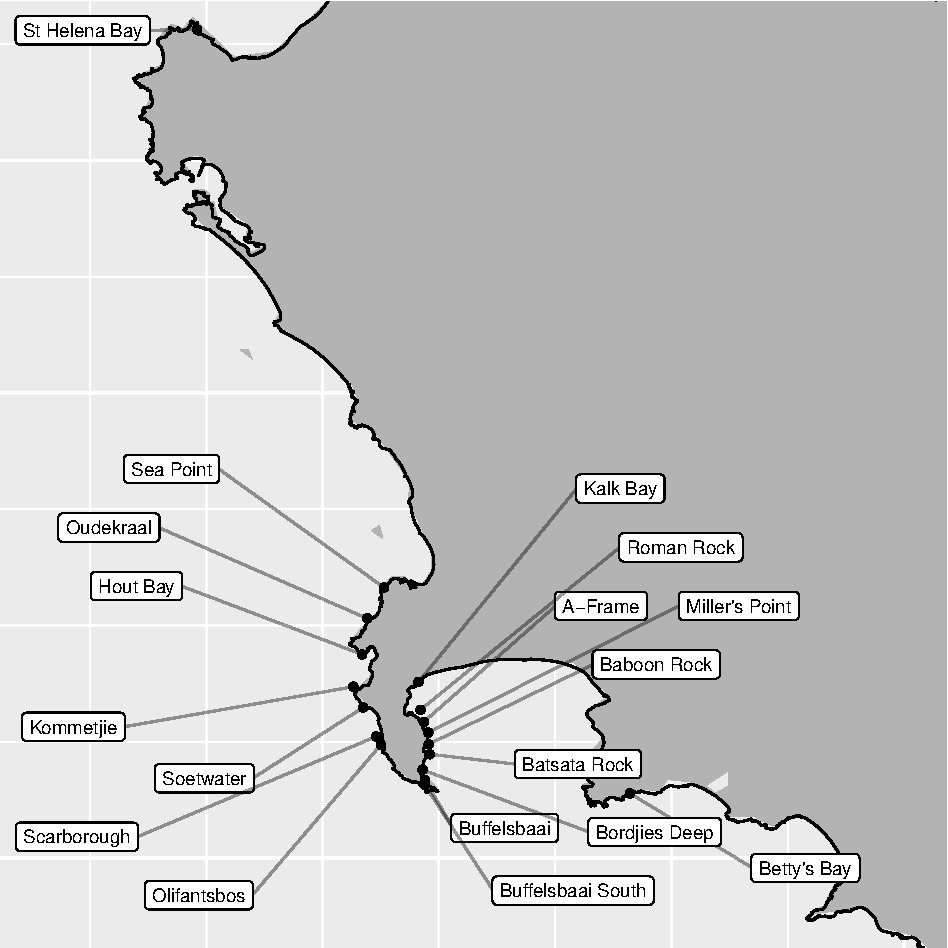
\includegraphics{thesis_chapter_3_files/figure-latex/unnamed-chunk-1-1.pdf}
\caption{Figure 2: Comparison of mean trajectories. Plot A is the
comparison of mean trajectories for only hydrodynamic drag and plot B is
the comparison of mean trajectories for simulations with varying degrees
of hydrodynamic and wind drag.}
\end{figure}

\hypertarget{comparison-of-density-distributions}{%
\subsection{Comparison of density
distributions}\label{comparison-of-density-distributions}}

Across all simulations particles flowed in a north-westward direction
(Figure 3). The density plots for simulations that considered any form
of drag showed a higher density of particles along the mean trajectory
path compared to the passive simulation which has an almost even density
of particles across grids (Figure 3A, 3E, 3I). In addition the density
plots show that the particles in simulations that considered any form of
drag got entrained in a vorticy while particles in the passive
simulation deflected away (Figure 3). Comparison of cross-sectional
areas and different drag exposure scenarios show no differences in mean
trajectory and spatial patterns in density, with only slight variations
across types.

\begin{figure}
\centering
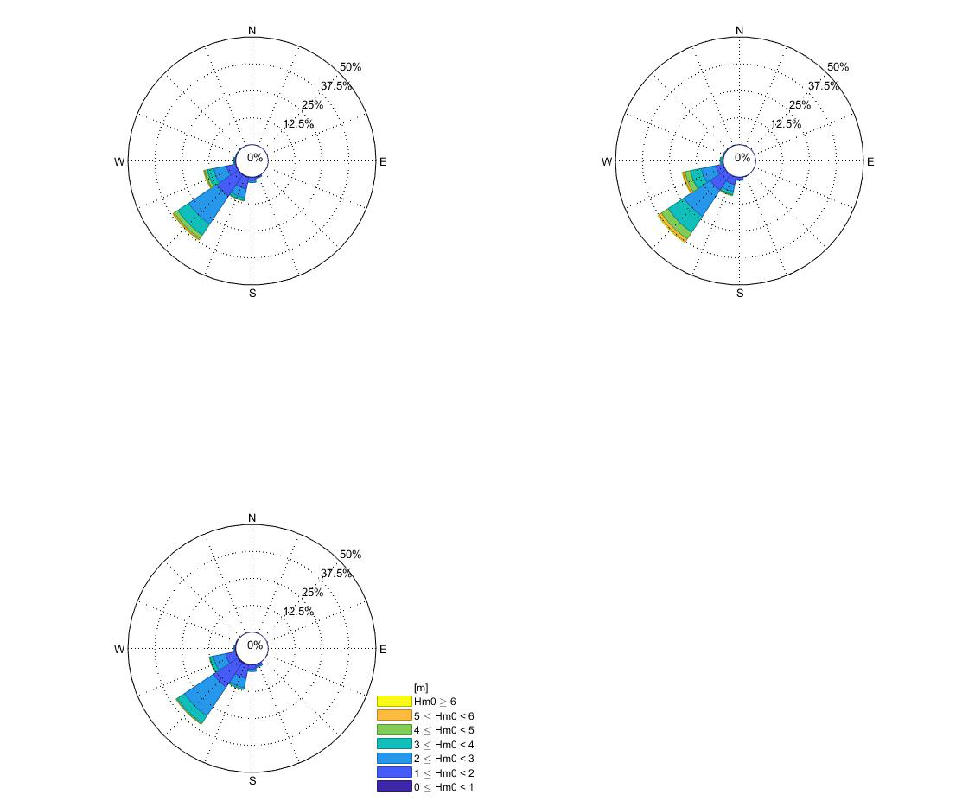
\includegraphics{thesis_chapter_3_files/figure-latex/unnamed-chunk-2-1.pdf}
\caption{Figure 3: Comparison of density of particles within each grid
cell for the end run time of each scenario. Plots A-D repressent the
minimum, plots E-H are the mean and plots I-L the maximum
cross-sectional areas. The bottom plot is the density plot for the
passive simulation.}
\end{figure}

\hypertarget{comparison-of-distances}{%
\subsection{Comparison of distances}\label{comparison-of-distances}}

There were significant differences among the median distances travelled
for all particles in each simulation (Figure 4; p \textless{} 0.05). The
simulations that considered for 100\% hydrodynamic drag travelled less
distance than particles for simulations which considered a combination
of hydrodynamic and wind drag scenarios. Comparison between simulations
that considered hydrodynamic and wind drag show no significant
differences with only slight variations among simulations.

\begin{figure}
\centering
\includegraphics{thesis_chapter_3_files/figure-latex/distance plot-1.pdf}
\caption{Figure 4: Boxplots of total distance of all particles from the
release site over the course of the simulation for each exposure
scenario.}
\end{figure}

\hypertarget{comparison-of-coefficents}{%
\subsection{Comparison of coefficents}\label{comparison-of-coefficents}}

The comparison of mean trajectories between the sphere and cylindrical
shape coefficients revealed no dissimilarity (Figure 5A). This was also
reflected when comparing distance travelled by particles and particle
density plots (Figure 5B). The simulation which used a cylindrical shape
coefficient showed higher density in an eddy compared to the simulation
which used a sphere for the shape coefficient (Figure 5C-D).

\begin{figure}
\centering
\includegraphics{thesis_chapter_3_files/figure-latex/shape data outputs-1.pdf}
\caption{Figure 5: Comparison of trajectory data between a kelp sphere
and kelp cylinder. Plot A is the comparison of mean trajectories, plot B
is the comparison of distance travelled by all particles, and plot C and
D are the density plots for simulations using a sphere and cylinderical
shape coefficient.}
\end{figure}

\hypertarget{discussion}{%
\section{Discussion}\label{discussion}}

The treatment of drifting macroalgae as purely lagrangian will not be
able to accurately determine patterns of passive dispersal, such as
entrainment in eddies or vortices (Fossette et al., 2012; Miron et al.,
2020). Although past research has shown the inclusion of inertia and
windage greatly increase observed macroalgae trajectory and entrainment
characteristics (Brooks et al., 2018, 2019; Putman et al., 2018, 2020),
current research has focused on large macroalgae-rafts which can vary
greatly in size and surface area. None of the past research has taken
advantage of the advancement in numerical ocean models and lagrangian
trajectory modeling to investigate how aspects of drag (hydrodynamic and
wind) affect the trajectory patterns of solitary drifting macroalgae.
This study compared particles trajectories with simulations that
included no forms of drag with simulations that included various forms
of both hydrodynamic and wind drag. The mean virtual kelp trajectory
deviated from the mean passive trajectory when including varying levels
of hydrodynamic and wind drag scenarios. The results from this study
show the inclusion of hydrodynamic and wind drag improves entrainment
patterns, and also our understanding of how surface area plays a role in
solitary drifting macroalgae trajectory, in this case \emph{E.maxima}.

Past research has inferred from direct and indirect techniques that
drifting macroalgae tend to follow the prevailing surface currents
(Hobday, 2000; Thiel and Gutow, 2005; Fraser et al., 2011; Rothäusler et
al., 2011, 2011). The results from this numerical experiment confirm
that drifting macroalgae do follow the surface current in the study
region when considering only hydrodynamic drag. In addition, not only
are the trajectories similar but so are the end points at the end of
simulation. However, when ad-hoc wind drag (windage) is considered in
combination with hydrodynamic drag the trajectories differ greatly when
compared to purely lagrangian particle trajectories. The inclusion of
wind drag causes the particles to flow further away from the coast and
with a greater distance travelled from the release location. The
difference in trajectory and distance covered can be attributed to the
inclusion of wind drag. Wind drag adds to the effects of hydrodynamic
drag when the wind direction and current direction are opposite to each
other. However, when the wind direction is in the same or similar
direction to that of the current, momentum energy from the wind is
transferred to the object (Hackett et al., 2006; Putman et al., 2020).
This causes the particles to travel further as well as exposed to
different time varying flows. Past studies have shown this when
including windage as a function of inertia (Putman et al., 2018, 2020;
Brooks et al., 2019). A study by Putman et al. (2020) used ad-hoc
windage factors that was based on the surface current velocity to assess
the approach for improving transport predictions of pelagic Sargassum.
The results showed that including ad-hoc windage factors improved
virtual trajectories compared to tracked Sargassum mats which was partly
due to the inclusion of momemtum energy transfer from wind. This is also
reflected in the analysis comparing distances travelled by all the
particles in each simulation. The particles in the simulations that
included wind drag traveled significantly greater distances compared to
the passive or hydrodynamic only drag.

The addition of drag forces into the simulation also causes the
particles to cluster together along the mean trajectory compared to that
of the passive particles which are more evenly dispersed. This is most
likely due to the shared drag characteristics among the particles which
included the plants weight and surface area into the calculation. Other
studies investigating flotsam trajectory characteristics have found
similar results (Breivik et al., 2011; Miron et al., 2020; Olascoaga et
al., 2020). A study by Miron et al. (2020) conducted field experiments
using a range of objects such as spheres, cubes, cuboids to compare to
investigate the effect of inertia on particles dynamics. The results
from the study showed that objects tended to cluster according to the
shape of the object which the authors attributed to shared
characteristics of inertia. Although drag forces were used in this study
and not inertia, the same conclusion applies, drag is an important
characteristic to consider when investigating or predicting solitary
drifting macroalgae.

The ocean is made up of varying time-varying flows and changes in an
objects velocity can cause the object to be exposed to different flow
patterns over time. The lack of dissimilarity between different
cross-sectional area types (minimum, mean and maximum) suggests that
reduction in velocity in relation to cross-sectional area is negligible.
A similar result was found by Le Gouvello et al. (2020) who investigated
the effects of swimming behavior on sea turtle hatchling dispersal in
the Agulhas region. The results suggested that the hatchlings
trajectories are mostly influenced by the ocean currents in the first
year of hatching due to low swimming speeds of juveniles. Therefore, the
differences in cross-sectional area types may not be significant enough
in order to have a significant effect on the relevant velocity vectors
(zonal and meridonal). Another possible reason is the resolution of the
ocean model used. The resolution of the underlying ocean model is an
important aspect of lagrangian ocean modeling and must be able to
resolve sub-grid scale ocean processes for finer scale applications. A
study by Hart-Davis et al. (2018) assessed the inclusion of stochastic
motion, wind and currents into forecasting for search and rescue using
the same model ocean model used in this study. The authors found that
the inclusion of brownian motion greatly increased the accuracy in
representing sub-grid scale processes and that the inclusion of wind,
currents and stochastic motion greatly improved forecasting
applications. Therefore, the authors argue that the lack of
dissimilarity between simulations of different cross-sectional area and
drag exposure scenarios is not as a result of the resolution of the
model.

The same is also true when comparing different hydrodynamic and wind
drag exposure scenarios. These scenarios reflect different buoyancy
situations which result in different amounts of surface area exposed to
hydrodynamic and/or wind drag. The similarities between the different
combined drag scenarios suggests that higher magnitudes of wind exposure
do not significantly alter trajectories. Instead, the results from this
study suggest that the inclusion of drag forces in simulating macroalgal
trajectory may result in improving accuracy of entrainment patterns. All
the simulations that included any form of drag resulted in a fairly high
density of particles entrained in a vortex. The entrainment and
expulsion from eddies and vortices is an important characteristic of
floating macroalgae. Accuracy in predicting entrainment and expulsion of
macroalgae-rafts from eddies has been investigated previously by Putman
et al. (2018) and Putman et al. (2020), who show that including windage
greatly improves entrainment patterns when comparing virtual and real
Sargassum rafts. However, the aforementioned studies investigated large
rafts and not floating individuals. Inertia is based on the size/weight
of the raft, while hydrodynamic and wind drag are based on current
velocity and surface area. Therefore, the role of inertia may be
negligible for a solitary individual and rather other forms of drag
should be considered. The results from this study suggest that the
inclusion of hydrodynamic and/or wind drag is an important component
when simulating virtual kelp particles will greatly increase the
accuracy of entrainment and expulsion from sub-grid mesoscale
oceanographic features, such as eddies and vortices. The use of a
cylindrical shape coefficient instead of a sphere in the calculation of
drag force also had no effect on the mean trajectory. Instead, the
inclusion of a different shape coefficient increased to the density of
particles entrained in an eddy field. This suggest that inclusion of
different shape coefficients play a role in further improving estimates
and hindcasts of macroalgal dispersal patterns.

\hypertarget{conclusion}{%
\section{Conclusion}\label{conclusion}}

Most of the past research has focused on large macroalgae rafts which
can vary greatly in size and shape, however no research exists
attempting to clarify the drifting characteristics of solitary
macroalgae. Understanding how to accurately model the distribution of
solitary kelp can lead to be understanding of accumulation zones and
sinks and ultimately the ecological links pertaining to those processes.
The findings from this study indicate that solitary floating virtual
\emph{E. maxima} particles tend to follow the prevailing surface
currents and the inclusion of wind causes the trajectories to differ
greatly from that of a purely lagrangian particle. Furthermore, the
inclusion of both hydrodynamic and wind drag cause clustering of
particles along the trajectory as well causing particles to become
entrained in eddies. Different cross-sectional areas exposed to
hydrodynamic and wind drag had no effect on overall trajectory
suggesting that those differences are negligible when investigating
dispersal patterns of drifting \emph{E.maxima}. In addition, the use of
a cylindrical shape coefficient has no effect on mean trajectory but
also causes higher density of particles to become entrained in an eddy.
Overall the inclusion of drag forces is an important aspect to consider
when investigating the dispersal patterns of solitary macroalgae, while
differences in cross-sectional areas are not. This study also provides
an approach which can be adapted to model any floating solitary
macroalgae, provided the surface area can be estimated accurately. Gaps
in the research exist when considering what oceanographic processes play
a role in solitary macroalgal dispersal as well as how these vary
seasonally. The identification of biological and physical factors that
play a role in accumulation zones is also needed, as well as better
estimates for sinking rates and raft-times.

\hypertarget{appendix}{%
\section{Appendix}\label{appendix}}

\hypertarget{domain-features}{%
\subsection{Domain features}\label{domain-features}}

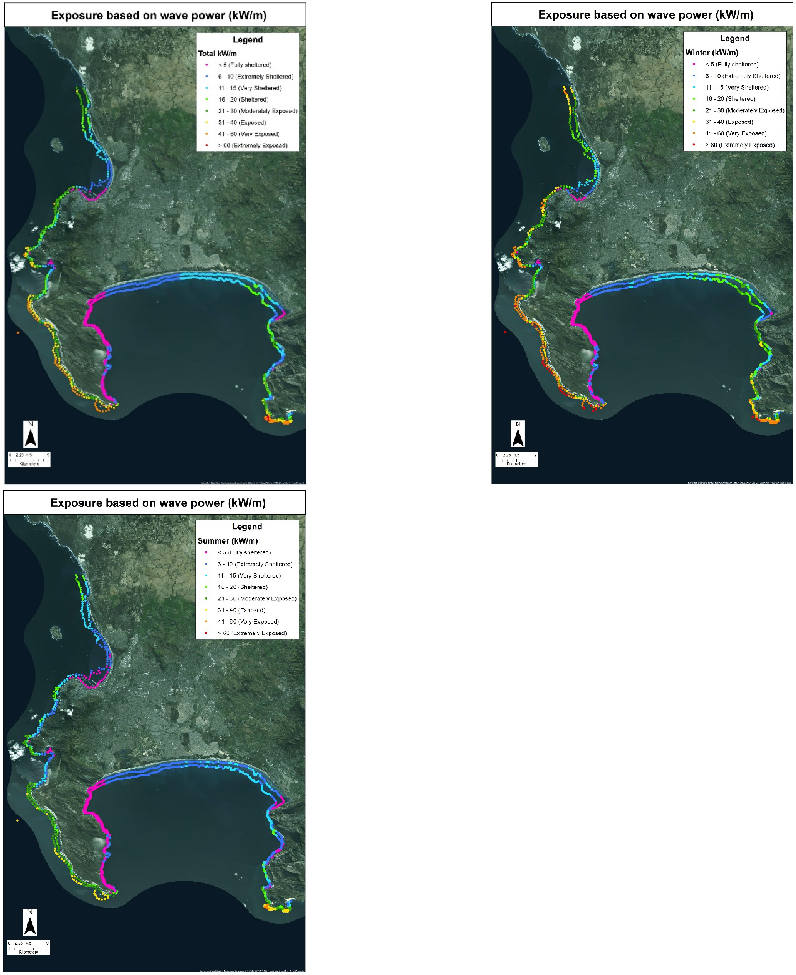
\includegraphics{thesis_chapter_3_files/figure-latex/unnamed-chunk-3-1.pdf}

\hypertarget{references}{%
\section*{References}\label{references}}
\addcontentsline{toc}{section}{References}

\hypertarget{refs}{}
\leavevmode\hypertarget{ref-allen1999}{}%
Allen, A., and Plourde, J. (1999). Review of leeway: Field experiments
and implementation. US coast guard rep.

\leavevmode\hypertarget{ref-andersson2017}{}%
Andersson, L. E., Scibilia, F., and Imsland, L. (2017). A study on an
iceberg drift trajectory. 8.
doi:\href{https://doi.org/10.1115/OMAE2017-62159}{10.1115/OMAE2017-62159}.

\leavevmode\hypertarget{ref-batista2018}{}%
Batista, M. B., Anderson, A. B., Sanches, P. F., Polito, P. S.,
Silveira, T. C. L., Velez-Rubio, G. M., et al. (2018). Kelps'
long-distance dispersal: role of ecological/oceanographic processes and
implications to marine forest conservation. \emph{Diversity} 10.
doi:\href{https://doi.org/10.3390/d10010011}{10.3390/d10010011}.

\leavevmode\hypertarget{ref-back2000}{}%
Bäck, S., Lehvo, A., and Blomster, J. (2000). Mass occurrence of
unattached \emph{enteromorpha intestinalis} on the finnish baltic sea
coast. 155--161.

\leavevmode\hypertarget{ref-beal2015}{}%
Beal, L. M., Elipot, S., Houk, A., and Leber, G. M. (2015). Capturing
the transport variability of a western boundary jet: Results from the
agulhas current time-series experiment (act). \emph{Journal of Physical
Oceanography} 45, 1302--1324.

\leavevmode\hypertarget{ref-blanke2002}{}%
Blanke, B., Roy, C., Penven, P., Speich, S., McWilliams, J., and Nelson,
G. (2002). Linking wind and interannual upwelling variability in a
regional model of the southern benguela. \emph{Geophysical Research
Letters} 29, 41--1.

\leavevmode\hypertarget{ref-blanke2005}{}%
Blanke, B., Speich, S., Bentamy, A., Roy, C., and Sow, B. (2005).
Modeling the structure and variability of the southern benguela
upwelling using quikscat wind forcing. \emph{Journal of Geophysical
Research: Oceans} 110.

\leavevmode\hypertarget{ref-breivik2011}{}%
Breivik, Ø., Allen, A. A., Maisondieu, C., and Roth, J. C. (2011).
Wind-induced drift of objects at sea: The leeway field method.
\emph{Applied Ocean Research} 33, 100--109.

\leavevmode\hypertarget{ref-brooks2019}{}%
Brooks, M. T., Coles, V. J., and Coles, W. C. (2019). Inertia influences
pelagic sargassum advection and distribution. \emph{Geophysical Research
Letters} 46, 2610--2618.

\leavevmode\hypertarget{ref-brooks2018}{}%
Brooks, M. T., Coles, V. J., Hood, R. R., and Gower, J. F. (2018).
Factors controlling the seasonal distribution of pelagic sargassum.
\emph{Marine Ecology Progress Series} 599, 1--18.

\leavevmode\hypertarget{ref-bushing1994}{}%
Bushing, W. W. (1994). Biogeographic and ecological implications of kelp
rafting as a dispersal vector for marine invertebrates. 22.

\leavevmode\hypertarget{ref-collins2010}{}%
Collins, C. J., Fraser, C. I., Ashcroft, A., and Waters, J. M. (2010).
Asymmetric dispersal of southern bull-kelp (\emph{Durvillaea
antarctica}) adults in coastal New Zealand: testing an oceanographic
hypothesis. \emph{Mol. Ecol.} 19, 4572--4580.

\leavevmode\hypertarget{ref-coppin2020}{}%
Coppin, R., Rautenbach, C., Ponton, T. J., and Smit, A. (2020).
Investigating waves and temperature as drivers of kelp morphology.
\emph{Frontiers in Marine Science} 7, 567.

\leavevmode\hypertarget{ref-dayton1985}{}%
Dayton, P. K. (1985). Ecology of Kelp Communities. \emph{Annual Review
of Ecology and Systematics} 16, 215--245.
doi:\href{https://doi.org/10.1146/annurev.es.16.110185.001243}{10.1146/annurev.es.16.110185.001243}.

\leavevmode\hypertarget{ref-delandmeter2019}{}%
Delandmeter, P., and Van Sebille, E. (2019). The parcels v2. 0
lagrangian framework: New field interpolation schemes.
\emph{Geoscientific Model Development} 12, 3571--3584.

\leavevmode\hypertarget{ref-dromgoole1982}{}%
Dromgoole, F. (1982). The buoyant properties of codium. \emph{Botanica
Marina} 25, 391--398.

\leavevmode\hypertarget{ref-edgar1987}{}%
Edgar, G. (1987). Dispersal of faunal and floral propagules associated
with drifting \emph{macrocystis pyrifera} plants. \emph{Marine Biology}
95, 599--610.

\leavevmode\hypertarget{ref-eik2009}{}%
Eik, K. (2009). Iceberg drift modelling and validation of applied
metocean hindcast data. \emph{Cold Regions Science and Technology} 57,
67--90.

\leavevmode\hypertarget{ref-fossette2012}{}%
Fossette, S., Putman, N. F., Lohmann, K. J., Marsh, R., and Hays, G. C.
(2012). A biologist's guide to assessing ocean currents: A review.
\emph{Marine Ecology Progress Series} 457, 285--301.

\leavevmode\hypertarget{ref-fraser2011}{}%
Fraser, C. I., Nikula, R., and Waters, J. M. (2011). Oceanic rafting by
a coastal community. \emph{Proceedings of the Royal Society B:
Biological Sciences} 278, 649--655.

\leavevmode\hypertarget{ref-garzoli1996}{}%
Garzoli, S. L., Gordon, A. L., Kamenkovich, V., Pillsbury, D., and
Duncombe-Rae, C. (1996). Variability and sources of the southeastern
atlantic circulation. \emph{Journal of Marine Research} 54, 1039--1071.

\leavevmode\hypertarget{ref-graiff2016}{}%
Graiff, A., Pantoja, J. F., Tala, F., and Thiel, M. (2016). Epibiont
load causes sinking of viable kelp rafts: Seasonal variation in floating
persistence of giant kelp \emph{macrocystis pyrifera}. \emph{Marine
biology} 163, 191.

\leavevmode\hypertarget{ref-griffin2017}{}%
Griffin, D., Oke, P., and Jones, E. (2017). \emph{The search for mh370
and ocean surface drift}. Commonwealth Scientific; Industrial Research
Organisation.

\leavevmode\hypertarget{ref-hackett2006}{}%
Hackett, B., Breivik, Ø., and Wettre, C. (2006). Forecasting the drift
of objects and substances in the ocean. 507--523.

\leavevmode\hypertarget{ref-hardman2003}{}%
Hardman-Mountford, N., Richardson, A., Agenbag, J., Hagen, E., Nykjaer,
L., Shillington, F., et al. (2003). Ocean climate of the south east
atlantic observed from satellite data and wind models. \emph{Progress in
Oceanography} 59, 181--221.

\leavevmode\hypertarget{ref-harrold1989}{}%
Harrold, C., and Lisin, S. (1989). Radio-tracking rafts of giant kelp:
Local production and regional transport. \emph{Journal of Experimental
Marine Biology and Ecology} 130, 237--251.

\leavevmode\hypertarget{ref-hart2018}{}%
Hart-Davis, M. G., Backeberg, B. C., and Bakhoday-Paskyabi, M. (2018).
An assessment of the importance of combining wind, ocean currents and
stochastic motions in a particle trajectory model for search and rescue
applications.

\leavevmode\hypertarget{ref-helmuth1994}{}%
Helmuth, B., Veit, R. R., and Holberton, R. (1994). Long-distance
dispersal of a subantarctic brooding bivalve \emph{(Gaimardia
trapesina)} by kelp-rafting. \emph{Marine biology} 120, 421--426.
doi:\href{https://doi.org/10.1007/BF00680216}{10.1007/BF00680216}.

\leavevmode\hypertarget{ref-hobday2000}{}%
Hobday, A. J. (2000). Age of drifting \emph{Macrocystis pyrifera} (L.)
C. Agardh rafts in the Southern California Bight. \emph{Journal of
experimental marine biology and ecology} 253, 97--114.
doi:\href{https://doi.org/10.1016/S0022-0981(00)00255-0}{10.1016/S0022-0981(00)00255-0}.

\leavevmode\hypertarget{ref-holmquist1994}{}%
Holmquist, J. (1994). Benthic macroalgae as a dispersal mechanism for
fauna: Influence of a marine tumbleweed. \emph{Journal of Experimental
Marine Biology and Ecology} 180, 235--251.

\leavevmode\hypertarget{ref-kingsford1995}{}%
Kingsford, M. J. (1995). Drift algae: A contribution to near-shore
habitat complexity in the pelagic environment and an attractant for
fish. \emph{Marine ecology progress series. Oldendorf} 116, 297--301.

\leavevmode\hypertarget{ref-gouvello2020}{}%
Le Gouvello, D. Z., Hart-Davis, M. G., Backeberg, B. C., and Nel, R.
(2020). Effects of swimming behaviour and oceanography on sea turtle
hatchling dispersal at the intersection of two ocean current systems.
\emph{Ecological Modelling} 431, 109130.

\leavevmode\hypertarget{ref-lichey2001}{}%
Lichey, C., and Hellmer, H. H. (2001). Modeling giant-iceberg drift
under the influence of sea ice in the weddell sea, antarctica.
\emph{Journal of Glaciology} 47, 452--460.

\leavevmode\hypertarget{ref-lutjeharms2007}{}%
Lutjeharms, J. (2007). Three decades of research on the greater agulhas
current.

\leavevmode\hypertarget{ref-lutjeharms2006}{}%
Lutjeharms, J. R. (2006). The agulhas current. 5.

\leavevmode\hypertarget{ref-lutjeharms1988}{}%
Lutjeharms, J., and Van Ballegooyen, R. (1988). The retroflection of the
agulhas current. \emph{Journal of Physical Oceanography} 18, 1570--1583.

\leavevmode\hypertarget{ref-macaya2005}{}%
Macaya, E. C., Boltana, S., Hinojosa, I. A., Macchiavello, J. E.,
Valdivia, N. A., Vasquez, N. R., et al. (2005). PRESENCE of sporophylls
in floating kelp rafts of macrocystis spp.(PHAEOPHYCEAE) along the
chilean pacific coast 1. \emph{Journal of Phycology} 41, 913--922.

\leavevmode\hypertarget{ref-McCormick2008}{}%
McCormick, T. B., Buckley, L. M., Brogan, J., and Perry, L. M. (2008).
Drift macroalgae as a potential dispersal mechanism for the white
abalone haliotis sorenseni. \emph{Marine Ecology Progress Series} 362,
225--232.

\leavevmode\hypertarget{ref-miron2020}{}%
Miron, P., Olascoaga, M., Beron-Vera, F., Putman, N., Triñanes, J.,
Lumpkin, R., et al. (2020). Clustering of marine-debris-and
sargassum-like drifters explained by inertial particle dynamics.
\emph{Geophysical Research Letters} 47, e2020GL089874.

\leavevmode\hypertarget{ref-nikula2013}{}%
Nikula, Spencer, and Waters (2013). Passive rafting is a powerful driver
of transoceanic gene flow. \emph{Biology letters} 9, 20120821.
doi:\href{https://doi.org/10.1098/rsbl.2012.0821}{10.1098/rsbl.2012.0821}.

\leavevmode\hypertarget{ref-norton1992}{}%
Norton, T. (1992). Dispersal by macroalgae. \emph{British Phycological
Journal} 27, 293--301.

\leavevmode\hypertarget{ref-olascoaga2020}{}%
Olascoaga, M. J., Beron-Vera, F. J., Miron, P., Triñanes, J., Putman,
N., Lumpkin, R., et al. (2020). Observation and quantification of
inertial effects on the drift of floating objects at the ocean surface.
\emph{Physics of Fluids} 32, 026601.

\leavevmode\hypertarget{ref-putman2018}{}%
Putman, N. F., Goni, G. J., Gramer, L. J., Hu, C., Johns, E. M.,
Trinanes, J., et al. (2018). Simulating transport pathways of pelagic
sargassum from the equatorial atlantic into the caribbean sea.
\emph{Progress in Oceanography} 165, 205--214.

\leavevmode\hypertarget{ref-putman2020}{}%
Putman, N. F., Lumpkin, R., Olascoaga, M. J., Trinanes, J., and Goni, G.
J. (2020). Improving transport predictions of pelagic sargassum.
\emph{Journal of Experimental Marine Biology and Ecology} 529, 151398.

\leavevmode\hypertarget{ref-rothausler2011}{}%
Rothäusler, E., Gómez, I., Hinojosa, I. A., Karsten, U., Miranda, L.,
Tala, F., et al. (2011). Kelp rafts in the humboldt current: Interplay
of abiotic and biotic factors limit their floating persistence and
dispersal potential. \emph{Limnology and oceanography} 56, 1751--1763.

\leavevmode\hypertarget{ref-rubio2009}{}%
Rubio, A., Blanke, B., Speich, S., Grima, N., and Roy, C. (2009).
Mesoscale eddy activity in the southern benguela upwelling system from
satellite altimetry and model data. \emph{Progress in Oceanography} 83,
288--295.

\leavevmode\hypertarget{ref-saunders2014}{}%
Saunders, G. W. (2014). Long distance kelp rafting impacts seaweed
biogeography in the Northeast Pacific: The kelp conveyor hypothesis.
\emph{Journal of phycology} 50, 968--974.
doi:\href{https://doi.org/10.1111/jpy.12237}{10.1111/jpy.12237}.

\leavevmode\hypertarget{ref-shannon1996}{}%
Shannon, L., and Nelson, G. (1996). The benguela: Large scale features
and processes and system variability. 163--210.

\leavevmode\hypertarget{ref-smith2002}{}%
Smith, S. D. A. (2002). Kelp rafts in the Southern Ocean. \emph{Global
ecology and biogeography: a journal of macroecology} 11, 67--69.
doi:\href{https://doi.org/10.1046/j.1466-822X.2001.00259.x}{10.1046/j.1466-822X.2001.00259.x}.

\leavevmode\hypertarget{ref-tala2013}{}%
Tala, F., Gómez, I., Luna-Jorquera, G., and Thiel, M. (2013).
Morphological, physiological and reproductive conditions of rafting bull
kelp \emph{(Durvillaea antarctica)} in northern-central Chile (30°S).
\emph{Marine biology} 160, 1339--1351.
doi:\href{https://doi.org/10.1007/s00227-013-2186-8}{10.1007/s00227-013-2186-8}.

\leavevmode\hypertarget{ref-tala2017}{}%
Tala, F., Penna-Díaz, M. A., Luna-Jorquera, G., Rothäusler, E., and
Thiel, M. (2017). Daily and seasonal changes of photobiological
responses in floating bull kelp \emph{Durvillaea antarctica} (Chamisso)
Hariot (Fucales: Phaeophyceae). \emph{Phycologia} 56, 271--283.

\leavevmode\hypertarget{ref-thiel2005}{}%
Thiel, M., and Gutow, L. (2005). The Ecology of rafting in the marine
environment. II. The rafting organisms and community. \emph{Oceanography
and Marine Biology: An Annual Review} 43, 279--418.

\leavevmode\hypertarget{ref-veitch2010}{}%
Veitch, J., Penven, P., and Shillington, F. (2010). Modeling equilibrium
dynamics of the benguela current system. \emph{Journal of Physical
Oceanography} 40, 1942--1964.

\leavevmode\hypertarget{ref-wichmann2012}{}%
Wichmann, C.-S., Hinojosa, I. A., and Thiel, M. (2012). Floating kelps
in Patagonian Fjords: an important vehicle for rafting invertebrates and
its relevance for biogeography. \emph{Mar. Biol.} 159, 2035--2049.
doi:\href{https://doi.org/10.1007/s00227-012-1990-x}{10.1007/s00227-012-1990-x}.

\end{document}
